\documentclass[10.5pt,a4paper]{article}
\usepackage[margin=2.4cm]{geometry}
\usepackage{amsmath,amssymb}
\usepackage{booktabs,array,multirow,tabularx}
\usepackage{graphicx,float,caption}
\usepackage{xcolor}
\usepackage{listings}
\usepackage{enumitem}
\usepackage{tikz}
\usetikzlibrary{arrows.meta,positioning}
\usepackage[colorlinks=true,linkcolor=teal!50!black,urlcolor=blue!50!black]{hyperref}
\usepackage{microtype}

\emergencystretch=4em
\setlist{itemsep=2pt,topsep=3pt,parsep=0pt}
\captionsetup{font=small,labelfont=bf}
\setlength{\parindent}{0pt}
\setlength{\parskip}{5pt}
\renewcommand{\arraystretch}{1.14}

\definecolor{cgood}{HTML}{0F766E}
\newcommand{\tx}[1]{\texttt{\detokenize{#1}}}
\lstset{basicstyle=\ttfamily\footnotesize,breaklines=true,frame=single,rulecolor=\color{black!25},
        backgroundcolor=\color{black!3},columns=fullflexible,keepspaces=true,showstringspaces=false}

\title{\textbf{Qwen3.5-4B on the Radeon RX 7900 XT:\\ 11{,}000 tokens/s INT4 Prefill and 200 tokens/s Decode}\\[4pt]
\large Rotated GPTQ-INT4 Inference with INT4 WMMA Kernels and a 236-Launch Decode Path on RDNA3}
\author{Sachin Mahesh\\ \texttt{sachinmahesh@berkeley.edu}\\ \href{https://github.com/SILVERTHRONE32}{github.com/SILVERTHRONE32}}
\date{November 2, 2026}

\begin{document}
\maketitle
\vspace{-0.9cm}

\begin{abstract}
\noindent
On a single Radeon RX~7900~XT, Qwen3.5-4B runs at 11{,}012\,tokens/s prefill (pp512) and 200.6\,tokens/s decode (tg128) with INT4 weights and 4-bit activations. This is 2.01$\times$ the prefill and
1.38$\times$ the decode throughput of Q4\_K\_M built from the same checkpoint and measured on the same build, and it places the RX~7900~XT third of eight GPUs compared (Section~\ref{sec:gpus}), ahead of the
RTX~5080 in prefill and level with it in decode. The default preset (8-bit activations) reaches 1.30$\times$ the prefill and 1.38$\times$ the decode throughput of Q4\_K\_M at the same perplexity degradation
(+1.9\% against +2.0\%) and a lower KL divergence from BF16 (0.024 against 0.028). The path stores every linear weight as a block-Hadamard-rotated, GPTQ-quantized symmetric INT4 tensor and evaluates it on
\tx{v_wmma_i32_16x16x16_iu4}; it transfers without modification to a fine-tune of the same backbone (Ossicle-4B), reproducing both the throughput and the accuracy ordering. Weights occupy a single copy in VRAM
(peak 3{,}358 against 3{,}621\,MiB), prefill uses a chunked WMMA gated-delta-net kernel and a WMMA flash-attention kernel for head size 256, and the decode graph was reduced from 847 to 236 kernel launches per token.
\end{abstract}

%=====================================================================================================================
\section{Introduction}

RDNA3 executes \tx{v_wmma_i32_16x16x16_iu4} at twice the rate of its iu8 counterpart. The quantized matrix-multiplication path of llama.cpp (MMQ) widens 4-bit weights to 8 bits and uses the iu8
instruction, reaching 36--40 integer TOPS on this device in our measurements. Using the INT4 pipeline directly requires 4-bit activations, and for unmodified models the channel-wise activation
outliers make that unusable. The present work combines three components:
\begin{enumerate}[label=(\roman*)]
\item a block-Hadamard rotation applied to both operands, which makes weights and activations close to Gaussian within each 256-element block;
\item GPTQ weight quantization in the rotated basis (symmetric INT4, one fp16 scale per 32 columns);
\item INT4 WMMA kernels that evaluate 8-bit activations as two INT4 passes and 4-bit activations as one, together with fused prefill and decode paths around them.
\end{enumerate}
We evaluate on the stock Qwen3.5-4B checkpoint (Section~\ref{sec:results}) and on Ossicle-4B, a fine-tune of the same backbone with an audio encoder, to establish that the result is not specific
to one set of weights (Section~\ref{sec:second}). Section~\ref{sec:decode} analyzes the decode path in detail; Section~\ref{sec:neg} lists what did not work.

%=====================================================================================================================
\section{Throughput relative to current GPUs}
\label{sec:gpus}

\begin{figure}[H]
\centering\includegraphics[width=.96\linewidth]{fig/sum_gpus.pdf}
\caption{Qwen3.5-4B, 4-bit quantization: prefill and decode throughput by GPU. RX~7900~XT: this work, INT4 \tx{fast}. Other GPUs: Local LLM Advisor leaderboard (llama.cpp, CUDA).}
\label{fig:gpus}
\end{figure}

\begin{table}[H]
\centering\fontsize{7.8}{9.3}\selectfont
\setlength{\tabcolsep}{3pt}
\begin{tabular*}{\linewidth}{@{\extracolsep{\fill}}lrrrrrr@{}}
\toprule
 & \multicolumn{2}{c}{Qwen3.5-4B} & \multicolumn{2}{c}{Qwen3.5-9B} & \multicolumn{2}{c}{Qwen3.8-27B}\\
GPU & prefill & decode & prefill & decode & prefill & decode\\
\midrule
RTX 5090 & 16{,}036 & 313.6 & 11{,}721 & 220.5 & 3{,}881 & 79\\
RTX 4090 & 14{,}882 & 220.2 & 9{,}762 & 141.6 & 3{,}417 & 51\\
\textbf{RX 7900 XT (INT4 \tx{fast}, this work)} & \textbf{11{,}012} & \textbf{200.6} & \textbf{6{,}581} & \textbf{125.8} & \textbf{2{,}013} & \textbf{50}\\
RTX 5080 & 10{,}057 & 200.5 & 6{,}543 & 136.1 & -- & 50\\
RTX 5070 Ti & 8{,}889 & 187.6 & 5{,}872 & 126.0 & -- & --\\
RTX 5070 & 7{,}449 & 154.5 & 4{,}652 & 101.3 & -- & --\\
RTX 3090 & 7{,}366 & 179.1 & 4{,}632 & 122.1 & 1{,}507 & 43\\
RTX 5060 Ti 16\,GB & 4{,}776 & 107.6 & 2{,}955 & 70.0 & -- & --\\
\bottomrule
\end{tabular*}
\caption{Qwen3.5-4B, Qwen3.5-9B and Qwen3.8-27B; local pp512/tg128, no MTP/speculation. 27B decode rounded to whole tokens/s; RTX~5080 27B: reported IQ4\_XS. -- = unavailable.}
\end{table}

The RX~7900~XT ranks third of the eight in both prefill and decode, behind the RTX~5090 and RTX~4090. Its prefill throughput is 1.09$\times$ that of the RTX~5080 and 1.50$\times$ that of the RTX~3090;
its decode throughput equals the RTX~5080's (200.6 against 200.5\,tokens/s) and is 1.12$\times$ the RTX~3090's. Against the RTX~4090 it reaches 0.74$\times$ the prefill and 0.91$\times$ the decode throughput.

%=====================================================================================================================
\section{Method}
\label{sec:method}

\begin{figure}[H]
\centering
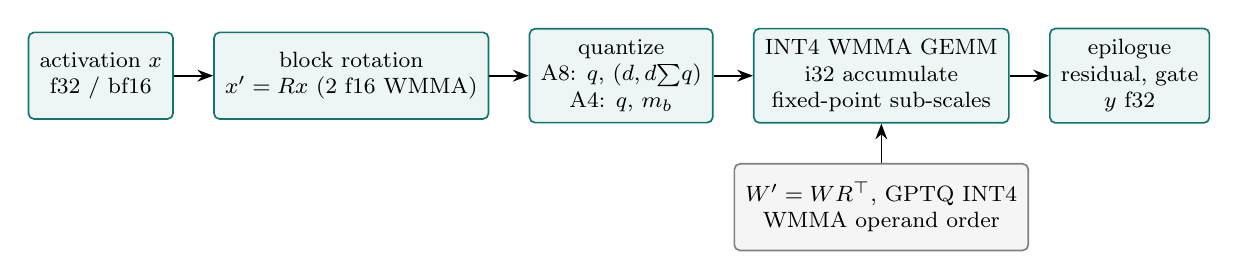
\begin{tikzpicture}[node distance=5mm,box/.style={draw=cgood,fill=cgood!7,rounded corners=2pt,minimum height=11mm,align=center,font=\footnotesize,line width=.6pt,inner sep=4pt},
  arr/.style={-{Stealth[length=2mm]},line width=.6pt}]
\node[box] (x) {activation $x$\\ f32 / bf16};
\node[box,right=of x] (r) {block rotation\\ $x'=Rx$ (2 f16 WMMA)};
\node[box,right=of r] (q) {quantize\\ A8: $q$, $(d,d\!\sum\!q)$\\ A4: $q$, $m_b$};
\node[box,right=of q] (g) {INT4 WMMA GEMM\\ i32 accumulate\\ fixed-point sub-scales};
\node[box,right=of g] (y) {epilogue\\ residual, gate\\ $y$ f32};
\node[box,below=5mm of g,fill=black!4,draw=black!50] (w) {$W'=WR^{\top}$, GPTQ INT4\\ WMMA operand order};
\draw[arr] (x)--(r); \draw[arr] (r)--(q); \draw[arr] (q)--(g); \draw[arr] (g)--(y); \draw[arr] (w)--(g);
\end{tikzpicture}
\caption{Dataflow of a rotated linear layer. Rotation, quantization and packing form a single fused kernel in prefill and are folded into the preceding normalization (or into the matvec itself) in decode.}
\end{figure}

\subsection{Rotation}
For an input dimension $K$ (a multiple of 256) define, per 256-block, $R=\tfrac1{16}H_{256}D$ with $H_{256}$ the Sylvester--Hadamard matrix and $D=\mathrm{diag}(s_j)$,
$s_j=-1$ if $((j\cdot2654435761)\bmod2^{32})\gg31$, else $+1$ (a hash, so converter and backend agree without storing the signs). $R$ is orthogonal, hence $W'x'=Wx$ for
$W'=WR^{\top}$ (applied blockwise along $K$) and $x'=Rx$. Weights are rotated offline; activations are rotated in the backend as $H_{16}\otimes H_{16}$ on a $16\times16$ view of each block,
i.e.\ two f16 WMMAs with the sign diagonal folded into the first operand.

\subsection{Weight quantization}
GPTQ is run in the rotated basis with Hessians accumulated by forward hooks on each of the 200 linear tensors in fp32 (128 sequences $\times$ 512 tokens of WikiText-2 train), Cholesky-inverse
error feedback (damping 0.01 of the mean diagonal, column blocks of 128), codes in $[-8,7]$ and one fp16 scale per 32 columns chosen by an MSE search over 26 candidates
$\{0.55,\ldots,1.05\}\cdot\max|w|/7$ on the error-compensated weights. The result is stored as ordinary Q4\_0 blocks; the token embedding/output head is Q6\_K. The mean relative weight error is
0.107 for both Qwen3.5-4B and Ossicle-4B. The loader recognizes a rotated file from the GGUF key \tx{ossicle.int4_rotation_block}. GPTQ takes about four minutes and 15\,GB of host memory.

\subsection{INT4 WMMA execution}
Weights are repacked into WMMA operand order with fixed-point integer sub-scales. The repacked layout has exactly the byte size of the Q4\_0 tensor, so each weight is converted \emph{in place}
at first use (through a temporary copy of one tensor at a time, before any graph is captured) and only one copy resides in VRAM.

\textbf{A8 (\tx{quality}).} An INT8 code $q\in[-128,127]$ is split as $q=16h+\ell$ with $h\in[-8,7]$ signed and $\ell\in[0,15]$ unsigned. The $h$ pass is accumulated, shifted by 4 bits, and the
$\ell$ pass is accumulated into the same accumulator before the integer sub-scale (fixed-point shift 12) is applied; the cross-unit accumulation is carried in f32 to avoid 24-bit integer overflow.
Two INT4 passes cost one INT8 pass, but on the faster pipe: 134 INT4-TOPS effective (74\% of the INT4 peak) against 36--40 TOPS for MMQ.

\textbf{A4 (\tx{fast}).} A single pass; the scale of each 256-block is the multiplier $m_b=\lceil16\,c\,\mathrm{amax}_b/\mathrm{amax}_{\text{token}}\rceil\in\{1,\ldots,16\}$ of $1/16$ of a per-token
reference, with clip $c=0.85$ (KLD 0.113 $\to$ 0.092 relative to $c=1$ in the clip sweep; $c=0.6$ gives 0.146), and weight sub-scales with shift 10. The weight scale group (32/64/128) is detected at load time.
A standalone kernel reaches 125 TOPS at scale-per-32 (149 at scale-per-128) against 182 TOPS for a pure-WMMA loop.

\begin{table}[H]
\centering\small
\begin{tabular}{@{}llll@{}}
\toprule
preset & activations & selection & decode\\
\midrule
\tx{quality} & INT8, two INT4 passes & default & INT8\\
\tx{fast} & INT4, one pass, clip 0.85 & \tx{GGML_INT4_PREFILL=fast} & INT8\\
\bottomrule
\end{tabular}
\caption{Presets. Decode (batch $\le8$) always uses 8-bit activations, so decode throughput does not depend on the preset.}
\end{table}

%=====================================================================================================================
\section{Experimental setup}

\textbf{Hardware and software.} One Radeon RX~7900~XT (gfx1100, wave32, 20\,GB, 254\,W cap), ROCm~10.1.0 from the pip wheels; llama.cpp fork \tx{llama.cpp-ossicle}, branch \tx{ossicle}, commit
\tx{bb04ca964} (branch \tx{decode/matvec-prologue-attn-fold}, on top of \tx{ad3d82c29}; Section~\ref{sec:decode}). All rows of every table were measured on the same build in one session.

\textbf{Baseline.} Q4\_K\_M quantized from the same BF16 GGUF with an importance matrix from WikiText-2 train (250 chunks of 1024 tokens).

\textbf{Accuracy.} Mean $D_{\mathrm{KL}}(P_{\mathrm{BF16}}\,\|\,P)$ over positions (``KLD''), perplexity ratio against the model's own BF16 GGUF, and same-top-1 rate, on 24 chunks of WikiText-2 test
(context 512, about 12{,}000 tokens); standard errors are those reported by \tx{llama-perplexity}.

\textbf{Throughput.} \tx{llama-bench}; prefill is the median of 8 runs after discarding the first (cold clocks), decode is \tx{tg128} from an empty context, median of 5. With a 128-token context (\tx{-d 128}) every decode figure is 1.4--2.2\,tokens/s higher.
Decode drifts by $\pm1.5$\,tokens/s with device temperature, so only same-session ratios are interpreted.

%=====================================================================================================================
\section{Results on Qwen3.5-4B}
\label{sec:results}

\begin{table}[H]
\centering\small
\begin{tabular}{@{}lrrrrrrr@{}}
\toprule
Qwen3.5-4B & pp512 & pp2048 & tg128 & $\Delta$PPL & KLD & top-1 & peak VRAM\\
 & \multicolumn{3}{c}{tokens/s} & \% & & \% & MiB\\
\midrule
Q4\_K\_M & 5{,}477 & 5{,}387 & 145.2 & $+2.00\pm0.35$ & $0.0278\pm0.0011$ & $91.9\pm0.3$ & 3{,}621\\
rotated INT4, \tx{quality} & 7{,}140 & 7{,}013 & 200.7 & $+1.92\pm0.40$ & $0.0241\pm0.0018$ & $92.7\pm0.3$ & 3{,}358\\
rotated INT4, \tx{fast} & 11{,}012 & 10{,}624 & 200.6 & $+8.67\pm0.74$ & $0.0969\pm0.0033$ & $86.1\pm0.4$ & 3{,}358$^{*}$\\
\bottomrule
\end{tabular}
\caption{Stock Qwen3.5-4B, one RX~7900~XT. $\Delta$PPL and KLD are against the BF16 GGUF (PPL 8.837). $^{*}$Measured for \tx{quality}; \tx{fast} uses the same weights.}
\label{tab:stock}
\end{table}

\begin{figure}[H]
\centering\includegraphics[width=.96\linewidth]{fig/sum_stock.pdf}
\caption{Stock Qwen3.5-4B; ratios are against Q4\_K\_M. Prefill: pp512. Decode: tg128.}
\end{figure}

\tx{quality} matches Q4\_K\_M in perplexity degradation (difference $-0.08$, well inside the standard errors) with a nominally lower KLD (0.0241 against 0.0278, a gap of about two standard errors unpaired) and a 0.8\,pp higher top-1
rate, at 1.30$\times$ prefill throughput at both pp512 and pp2048, 1.38$\times$ decode throughput and 7\% lower peak VRAM. We do not claim an accuracy advantage over Q4\_K\_M; the result is equal accuracy at higher throughput.
\tx{fast} reaches 2.01$\times$ (pp512) and 1.97$\times$ (pp2048) prefill throughput; its KLD is 3.5$\times$ that of Q4\_K\_M and its perplexity degradation 8.7\%. Moving the activations from 8 to 4 bits accounts for the
entire difference between the presets (KLD 0.024 $\to$ 0.097), consistent with the per-tensor-kind simulation in the technical report, in which the FFN projections and the GDN output projection dominate the 4-bit-activation cost.

\subsection{A second model: Ossicle-4B}
\label{sec:second}
Ossicle-4B shares the backbone and architecture (24 gated-delta-net and 8 full-attention layers, hidden size 2560) and adds an audio encoder; its language weights are a fine-tune. The identical pipeline
(Section~\ref{sec:repro}) was applied to both checkpoints; the only change was extending the GPTQ script to read the original checkpoint's tensor names.

\begin{table}[H]
\centering\small
\begin{tabular}{@{}llrrrrrr@{}}
\toprule
model & format & pp512 & pp2048 & tg128 & $\Delta$PPL (\%) & KLD & top-1 (\%)\\
\midrule
\multirow{3}{*}{Qwen3.5-4B} & Q4\_K\_M & 5{,}477 & 5{,}387 & 145.2 & $+2.00\pm0.35$ & $0.0278\pm0.0011$ & 91.9\\
 & INT4 \tx{quality} & 7{,}140 & 7{,}013 & 200.7 & $+1.92\pm0.40$ & $0.0241\pm0.0018$ & 92.7\\
 & INT4 \tx{fast} & 11{,}012 & 10{,}624 & 200.6 & $+8.67\pm0.74$ & $0.0969\pm0.0033$ & 86.1\\
\midrule
\multirow{3}{*}{Ossicle-4B} & Q4\_K\_M & 5{,}461 & 5{,}356 & 145.0 & $+3.51\pm0.42$ & $0.0311\pm0.0015$ & 91.2\\
 & INT4 \tx{quality} & 7{,}094 & 6{,}992 & 200.6 & $+2.02\pm0.37$ & $0.0250\pm0.0014$ & 92.3\\
 & INT4 \tx{fast} & 10{,}934 & 10{,}606 & 200.6 & $+9.11\pm0.79$ & $0.1006\pm0.0036$ & 85.0\\
\bottomrule
\end{tabular}
\caption{Both models, one pipeline, one build; accuracy against each model's own BF16 original (PPL 8.837 and 9.475).}
\end{table}

\begin{figure}[H]
\centering\includegraphics[width=.62\linewidth]{fig/sum_plane.pdf}
\caption{Prefill throughput (pp512) against KLD. Circles: Qwen3.5-4B; squares: Ossicle-4B.}
\end{figure}

Throughput agrees within 0.7\% between the models for every format, as expected for identical tensor shapes. The accuracy ordering is the same: \tx{quality} below Q4\_K\_M in KLD (ratio 0.87 for Qwen3.5-4B, 0.80 for
Ossicle-4B) and \tx{fast} at 3.5$\times$ and 3.2$\times$ Q4\_K\_M. Both models are 4B members of one architecture family; other families and sizes were not measured.

\subsection{Speculative decoding}
Qwen3.5 checkpoints carry a one-layer MTP head, used as a draft model (\tx{--spec-type draft-mtp}) with a 0.50\,GB head file (Q8\_0 layer, Q4\_K embedding/output). With two drafts under \tx{llama-server} and greedy sampling, the output is identical to plain
decoding. Ossicle-4B: 190.7 $\to$ 229\,tokens/s (71\% acceptance, build \tx{ae36245f8}); stock Qwen3.5-4B: 168.5 $\to$ 218.8\,tokens/s (64\%, build \tx{72ec3b93e}). These were measured on earlier builds
than the tables above and were not repeated on the final one.

%=====================================================================================================================
\section{Prefill path}

The GEMM runs at about 74\% of the INT4 peak at A8; tile shapes (MI,NJ,waves) $(2,2,4)$, $(2,2,16)$, $(1,2,8)$ differ by under 2\%. Beyond the GEMM, a 512-token \tx{fast} pass is dominated by the operations below, each of which was
replaced or fused (Ossicle-4B, pp512 on the builds of the time).

\begin{itemize}
\item \textbf{Chunked WY gated-delta-net on WMMA.} A prep kernel (parallel over chunk$\times$head) forms $A=\mathrm{tril}(\beta_je^{g_j-g_i}k_j\!\cdot\!k_i)$ and $P=\mathrm{tril}(e^{g_t-g_j}q_t\!\cdot\!k_j)$ with f16 WMMA and solves
$(I+A)X=[\beta v\,|\,\beta e^{g}k]$ in 16-row panels (WMMA for off-diagonal updates, f32 for the diagonal blocks); a scan kernel, sequential over chunks and parallel over heads$\times$16 state columns, keeps the f32 state in WMMA
accumulators. 0.46 $\to$ 0.14\,ms per layer per 512 tokens; relative RMS error against an f64 recurrence $1.6$--$2.5\cdot10^{-4}$ per layer. A scalar-code version of the same algebra was 9--42\% slower than the recurrent kernel; the gain
required ISA-level work (branch-free preloads, no \tx{vmcnt(0)} per load).
\item \textbf{WMMA flash attention, head size 256.} The upstream WMMA path is excluded for RDNA3 at this head size (errors of order $10^{-2}$); the new kernel (64 rows = tokens$\times$GQA heads per block, 8 waves with the head dimension
split over wave pairs, Q in LDS, K and V$^{\top}$ tiles through one LDS buffer with conflict-free transposed V writes, mask-driven tile skipping, heaviest causal blocks first) takes a pp2048 pass from 25.5 to 12.0\,ms; all 2{,}920
\tx{FLASH_ATTN_EXT} tests pass.
\item \textbf{Fusion.} Shared activation packing across sibling matmuls (qkv+z, q/k/v, gate/up), SwiGLU and SiLU$\cdot$mul inside the pack kernel, the residual add in the GEMM epilogue, GDN $\alpha/\beta$ (convert, hipBLASLt, convert $\to$ one skinny bf16 WMMA
kernel with sigmoid / softplus$\cdot A$ epilogue), paired q/k L2 norms, a tiled LDS-transpose conv concat (1.8 $\to$ 0.6\,ms), and removal of three memsets per GEMM.
\end{itemize}

\begin{table}[H]
\centering\small
\begin{tabular}{@{}p{8.2cm}rrrr@{}}
\toprule
 & \multicolumn{2}{c}{\tx{quality}} & \multicolumn{2}{c}{\tx{fast}}\\
step (cumulative) & pp512 & pp2048 & pp512 & pp2048\\
\midrule
single-copy weights (baseline of this round) & 5{,}836 & 5{,}644 & 8{,}212 & 7{,}773\\
chunked WMMA gated-delta-net & 6{,}369 & 6{,}106 & 9{,}208 & 8{,}721\\
shared packing, GLU in pack kernel, tiled concat & 6{,}744 & 6{,}489 & 10{,}090 & 9{,}501\\
WMMA attention, GEMM residual epilogue, skinny gate kernel & 6{,}945 & 6{,}885 & 10{,}457 & 10{,}333\\
gate epilogue, paired L2 norm, 128-thread head norms & 7{,}082 & 6{,}991 & 10{,}895 & 10{,}570\\
\bottomrule
\end{tabular}
\caption{Prefill throughput (tokens/s) by optimization step, Ossicle-4B. KLD (0.0250) and MMAU did not change at any step; the fusions are bit-identical to the unfused path.}
\end{table}

%=====================================================================================================================
\section{Decode path}
\label{sec:decode}

A decode token reads 2.53\,GB of weights (2.0\,GB of body weights, 0.52\,GB Q6\_K head), i.e.\ 3.37\,ms at 750\,GB/s, an upper bound of about 297\,tokens/s. The first complete INT4 decode path (not the Q4\_K\_M baseline) ran at 138.3\,tokens/s on an earlier build, at 64\% device occupancy, with 847 launches per token
and $\approx$3.1\,\textmu s of idle time after each, while the matvecs already streamed at 90\% of the bandwidth bound; the work was therefore launch reduction. On the final build, Q4\_K\_M decodes at 145.2\,tokens/s. The matvec (\tx{k_mv}) operates on the repacked layout: one block is 16 weight
rows $\times$ 10 waves splitting the 256-blocks of $K$ (10 divides the 10 super-blocks of $K=2560$).

\begin{figure}[!ht]
\centering\includegraphics[width=.7\linewidth]{fig/sum_decode.pdf}
\caption{Decode throughput against launches per token (Ossicle-4B and Qwen3.5-4B share the graph; readings from different sessions, empty context). The leftmost point is the first complete INT4 decode path (847 launches, 138.3\,tokens/s, earlier build), not the Q4\_K\_M baseline (145.2\,tokens/s on the final build). Dashed: the bandwidth bound.}
\end{figure}

\begin{table}[!ht]
\centering\small
\begin{tabularx}{\linewidth}{@{}>{\raggedright\arraybackslash}Xrr@{}}
\toprule
fusion (cumulative) & launches/token & tokens/s\\
\midrule
first complete INT4 decode path (earlier build) & 847 & 138.3\\
rotation shared by sibling matvecs; residual add in the matvec epilogue & 732 & 143.3\\
RMSNorm fused with rotation + INT8 quantization; SiLU(z)$\cdot$norm folded into the \tx{ssm_out} matvec rotation; 10-wave blocks & 620 & 155.0\\
GDN state read in place from the cache row; conv cluster (gather, concat, cpy, \tx{ssm_conv}, SiLU) as one kernel & 524 & 166.9\\
GDN $\alpha{+}\beta$ in one launch; q/k L2 norm inside the GDN decode kernel; rotation inside the matvec for single-consumer inputs & 412 & 173.9\\
DPP reductions in the rotate/quantize prologues; attention gate and per-head norm folded into the matvec rotations & 348 & 186.1\\
q/k RMSNorm + multi-section RoPE + K/V write in one launch per attention layer & 308 & 190.8\\
conv cluster in the epilogue of the qkv matvec & 284 & 193.2\\
GDN z-projection shares the qkv launch & 260 & 195.5\\
attention q, k, v in one launch; register-resident norm kernel; 8-column gate matvec as two launches of 4 & 244 & 199.4\\
matvec prologue and in-kernel attention combine (below) & 236 & 200.7\\
\bottomrule
\end{tabularx}
\caption{Decode fusion steps (tg128, empty context); readings from different sessions; last row: stock Qwen3.5-4B, \tx{quality}.}
\end{table}

\subsection{Profile of the final build (236 launches)}
\begin{figure}[H]
\centering\includegraphics[width=.8\linewidth]{fig/decode_breakdown.pdf}
\caption{Kernel time per token on the final build (236 launches; stock Qwen3.5-4B, \tx{rocprofv3}, last 100 tokens of one trace; tracing inflates a token by about 7\%). Launch counts in brackets.}
\end{figure}
\begin{table}[H]
\centering\small
\begin{tabular}{@{}lrrrrr@{}}
\toprule
kernel & calls & \textmu s/call & \textmu s/token & share of busy & GB/s\\
\midrule
FFN gate+up (26.5\,MB) & 32 & 38.9 & 1{,}245 & 28.8\% & 683\\
LM head, Q6\_K (521\,MB) & 1 & 664 & 664 & 15.3\% & 785\\
FFN down (13.3\,MB) & 32 & 20.2 & 646 & 14.9\% & 658\\
GDN qkv+z (17.7\,MB) & 24 & 25.0 & 600 & 13.9\% & 708\\
GDN \tx{ssm_out}, in-kernel rotation (5.9\,MB) & 24 & 15.6 & 374 & 8.6\% & 379\\
RMSNorm + rotation + quantization & 64 & 3.6 & 229 & 5.3\% & --\\
GDN recurrence & 24 & 8.3 & 199 & 4.6\% & --\\
attention q+k+v (14.7\,MB) & 8 & 20.8 & 166 & 3.8\% & 710\\
attention \tx{attn_output}, in-kernel rotation (5.9\,MB) & 8 & 13.0 & 104 & 2.4\% & 455\\
attention tile + prep & 16 & -- & 95 & 2.2\% & --\\
\bottomrule
\end{tabular}
\caption{Decode kernel profile of the final build (236 launches; one trace, stock Qwen3.5-4B, last 100 tokens): 5{,}347\,\textmu s per traced token, of which 4{,}327\,\textmu s is kernel time and 1{,}020\,\textmu s (19\%) idle time between launches. Shares are of kernel time.}
\end{table}

Kernels that stream large weights run at 660--790\,GB/s. The remainder is launch gaps and two latency-bound projections ($K=4096$: \tx{ssm_out}, \tx{attn_output}) whose input is the preceding kernel's output. An ablation of \tx{ssm_out}, run before the two changes below (15.8\,\textmu s), separates the components: constants in place of weight loads 8.2\,\textmu s; no rotation 12.7\,\textmu s; neither 3.1\,\textmu s (launch, dot product, epilogue). The weight stream alone costs 9.6\,\textmu s (615\,GB/s against
a 7.9\,\textmu s bound) and the rotation prologue adds about 2.8\,\textmu s that the stream does not hide. Two changes address this and the attention tail; the profile above already includes them.

\textbf{Matvec prologue.} Each of the 160 blocks rotates and quantizes the full activation, one 256-block per wave. The quantizer performed eight dependent max/sum reduction pairs with a divergent lane-0 store between them; the eight
reductions are independent and now execute in lock-step on DPP, with a single scale store, and the per-row scale and residual loads are issued at kernel start. Per-call times fall by 0.4--0.6\,\textmu s for \tx{ssm_out},
\tx{ffn_down} and \tx{attn_output}, and by 0.15\,\textmu s for the 64 normalization kernels (197.2 $\to$ 199.4\,tokens/s, interleaved A/B).

\textbf{In-kernel attention combine.} The split-KV decode attention launched \tx{flash_attn_combine_results} (2.2\,\textmu s plus a 3.1\,\textmu s gap) in each of the 8 attention layers. The last block to finish each (tile, head-group)
combines the group's partial results: release fence, atomic increment of a counter in a zero-initialized device array that the last block resets (no per-launch memset or allocation), acquire fence, then one warp per head row with
lane $l$ reading the metadata of parallel block $l$ and eight contiguous outputs per lane. A first version with dependent scalar coherent loads lengthened the tile kernel by 17\,\textmu s and reduced throughput; the warp-per-row version adds
1.9\,\textmu s (7.0 $\to$ 8.9\,\textmu s) and removes the launch. It applies to a single query token, at most 32 parallel blocks and $d_v\bmod128=0$, on HIP only (\tx{GGML_FA_FOLD=0} disables it). Throughput by context depth (tokens):
198.6/199.3 at 0, 200.8/201.5 at 128, 199.2/199.7 at 512, 195.1/195.2 at 2048 and 188.4/188.0 at 6000 (fold off/on), i.e.\ a gain of 0.5--0.7\,tokens/s at short context that vanishes by 2k tokens.

Both changes together: 197.5 $\to$ 199.7 (empty context) and 199.4 $\to$ 201.6 (128-token context) for Ossicle-4B. Batch-8 and prefill-path KLD/PPL are bit-identical to the preceding commit; at batch 1 PPL changes by $+0.0010$ and
KLD by $-0.0002$ (rounding-level, from different FMA contraction in the epilogue). Prefill throughput is unchanged. The remaining overhead is $\approx$1\,ms of launch gaps (236 launches), the $K=4096$ projections, and the GDN recurrence (8.2\,\textmu s
against about 5.3\,\textmu s for its state traffic).

%=====================================================================================================================
\section{Negative and neutral results}
\label{sec:neg}

\begin{table}[H]
\centering\small
\begin{tabularx}{\linewidth}{@{}>{\raggedright\arraybackslash}p{6.0cm}X@{}}
\toprule
experiment & outcome (tokens/s unless stated)\\
\midrule
Scalar-code chunked WY gated-delta-net & correct, 9--42\% slower than the recurrent kernel\\
NVFP4/MXFP4 re-gridded to uniform INT4 & +0.07 KLD, no gain over BF16 $\to$ INT4\\
Sparsity skipping in the GEMM & exact; 0--6\% of real tiles skippable\\
Scale groups of 64/128 & +5\% prefill for +0.005--0.015 KLD\\
Next-block weight prefetch in the in-kernel-rotation matvec & 169.6--188.6 against 194.7--196.5 (VGPRs 112 $\to$ 128)\\
Rotation input requested before the weights & 195.3 against 197.7\\
First weight loads issued before constant setup & 194.4 against 199.6\\
Wave count $\ne10$ (rotation matvec: $K{=}4096$ at 5, 8, 16; $K{=}9216$ at 9, 12, 18) & 188--191 against 195.6; gate/up kernel at 1, 2, 5 waves: no gain\\
Rotation constants as lane masks ($\sim$95 fewer VALU operations) & neutral (199.65 against 199.8): the prologue is latency-bound\\
Single-block attention at short context (no combine) & slower at every depth (196.8 against 199.4 at depth 0)\\
Fused FFN, one launch with a grid barrier & 191.7 against 196.9\\
Output norm and quantization fused before the head & 193.3 against 198.7\\
Weight prefetch into the Infinity Cache from a side stream (8/24/40\,MB) & 181/136/105 against 186\\
\bottomrule
\end{tabularx}
\caption{Experiments not retained. Every variant that raised the rotation matvec from 112 to 128 VGPRs lost 1--5\%.}
\end{table}

%=====================================================================================================================
\section{Reproduction on stock Qwen3.5-4B}
\label{sec:repro}

Requirements: an RDNA3 GPU (tested: RX~7900~XT, ROCm~10.1.0), 15\,GB of host memory for GPTQ, about 20\,GB of disk, WikiText-2 raw files.

\begin{lstlisting}[language=bash]
# fork with the INT4 path (branch "decode/matvec-prologue-attn-fold" = "ossicle" plus the decode commits), built for gfx1100
cmake -S . -B build -DGGML_HIP=ON -DAMDGPU_TARGETS=gfx1100 -DCMAKE_BUILD_TYPE=Release && cmake --build build -j

# BF16 GGUF from the unmodified checkpoint
huggingface-cli download Qwen/Qwen3.5-4B --local-dir qwen35-4b
python convert_hf_to_gguf.py qwen35-4b --outtype bf16 --no-mtp --outfile qwen35-4b-bf16.gguf

# GPTQ in the rotated basis (about 4 min, 15 GB RAM; calibration: WikiText-2 train)
python scripts/gptq_rotate.py --src qwen35-4b --out gptq_g32.safetensors --group 32 --calib 128

# rotated GGUF (per-tensor check against the BF16 weights; Q6_K output head)
python scripts/rotate_quantize.py qwen35-4b-bf16.gguf qwen35-4b-rotq4-gptq.gguf --blocks gptq_g32.safetensors --embd q6_k

# run
llama-server -m qwen35-4b-rotq4-gptq.gguf -ngl 99                           # quality
GGML_INT4_PREFILL=fast llama-server -m qwen35-4b-rotq4-gptq.gguf -ngl 99    # fast

# measure
llama-bench -m qwen35-4b-rotq4-gptq.gguf -ngl 99 -p 512,2048 -n 128 -d 0,128 -r 9
llama-perplexity -m qwen35-4b-bf16.gguf -f wiki.test.raw -c 512 -ngl 99 --chunks 24 --kl-divergence-base base.bin     # BF16 reference
llama-perplexity -m qwen35-4b-rotq4-gptq.gguf -f wiki.test.raw -c 512 -ngl 99 --chunks 24 --kl-divergence-base base.bin --kl-divergence
\end{lstlisting}

The Q4\_K\_M baseline: \tx{llama-imatrix} on the BF16 GGUF (WikiText-2 train, \tx{-c 1024 --chunks 250}), then \tx{llama-quantize} with that matrix, measured with the same commands.

%=====================================================================================================================
\section{Limitations}

\begin{itemize}
\item \textbf{Target.} RDNA3 only (gfx1100 tested). The files are not interchangeable with Q4\_0: any other backend decodes the rotated codes as unrotated and produces garbage.
\item \textbf{Scope.} Two models, both 4B members of the Qwen3.5 architecture. Other families and sizes are untested, and the decode analysis is specific to this architecture's layer mix.
\item \textbf{\tx{fast}.} 2.0$\times$ prefill for $\Delta$PPL $+8.7\%$ and KLD 0.097; it is not equivalent to \tx{quality}.
\item \textbf{GPU comparison.} The comparison with the RTX~5080 and the other GPUs in Section~\ref{sec:gpus} is not like-for-like. The INT4 \tx{fast} path has a higher perplexity and KLD than standard Q4 quantizations (Section~\ref{sec:results}), and the leaderboard publishes neither its prompt length nor its other benchmark settings (only a Q4 quantization class), so the two sets of throughput figures were not obtained under identical conditions.
\item \textbf{Calibration and metrics.} GPTQ calibration is text only; accuracy is reported on WikiText-2 (24 chunks), with no downstream benchmark for the stock model.
\item \textbf{Measurement.} Decode throughput varies by $\pm1.5$\,tokens/s with device temperature; baselines are therefore taken in the same session. Decode-path KLD references cover 4 chunks. The in-kernel combine is HIP-only and keeps 16\,KB of static
device counters. The speculative-decoding figures predate the final build.
\item \textbf{Untested.} Multi-GPU, repeated load/unload in one process, and partial offload.
\end{itemize}

\section*{Artifacts}
\sloppy
Fork \tx{SILVERTHRONE32/llama.cpp-ossicle}, branch \tx{ossicle} (decode series \tx{8546fe90a}\ldots\tx{ad3d82c29}) and branch \tx{decode/matvec-prologue-attn-fold} (\tx{e96773ca4}, \tx{bb04ca964}: the matvec prologue and the in-kernel attention combine);
files \tx{SILVERTHRONE/Ossicle-4B-GGUF} (stock model: \tx{rdna3/qwen35-4b-rotq4-gptq.gguf}). License: Apache~2.0. The full technical report (Ossicle-4B, all experiments and caveats) accompanies this document.

\section*{Affiliation}
This work was carried out independently of the author's university. UC Berkeley had no role in it, and the university email address is provided for contact only.

\end{document}
